\documentclass{article}

% Remember to change this and recompile before use!
\def\today{20 Jan 2024}
\def\lectureno{8-9}
\def\classname{MATH5.1EL}

\usepackage{amsmath}
\usepackage{amsthm}
\usepackage[utf8]{inputenc}
\usepackage{xcolor}
\usepackage{tikz}
\usepackage{tkz-euclide}
\usepackage{lmodern}
\usepackage[normalem]{ulem}
\usepackage{float}
\usepackage{fancyhdr}
%\usepackage{showframe}
\usepackage{mdframed}
\usetikzlibrary{calc,intersections}
\tikzset{new/.style={color=red},small label/.style={font=\scriptsize},node label/.style={}}

\title{\classname \\ Introduction to Euclidean Geometry}
\author{T Yeung}
\date{\today}

\DeclareMathOperator{\Pow}{Pow}
\newtheorem{theorem}{Theorem}[section]
\newtheorem{corollary}{Corollary}[theorem]
\theoremstyle{definition}
\newtheorem{question}{Question}

\begin{document}
\pagestyle{fancy}
\fancyhead{}\fancyfoot{}
\fancyhead[L]{\classname}
\fancyhead[C]{L\lectureno}
\fancyhead[R]{\today}

\maketitle

\section{Introduction}

In the vast tapestry of mathematical exploration, few realms evoke a sense of elegance and timeless beauty quite like Euclidean geometry. With its origins deeply rooted in ancient Greece, this branch of mathematics has captivated the hearts and minds of scholars and thinkers for centuries.
\section{Motivation}
\noindent
\begin{minipage}{0.6\textwidth}
Given
\begin{itemize}
	\item $\angle DAC=30^\circ$
	\item $\angle CDB=40^\circ$
	\item $\angle ABD=50^\circ$
	\item $DB \perp AC$
\end{itemize}
What angles can you find?
\end{minipage}
\begin{minipage}{0.38\textwidth}
\centering
\begin{figure}[H]
	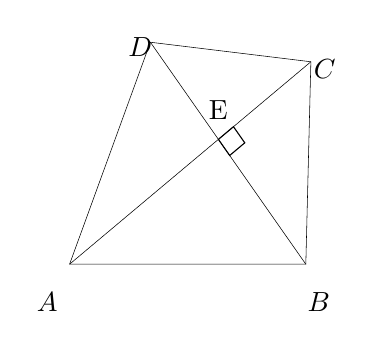
\begin{tikzpicture}
		\tkzDefPoint(0,0){A}
		\tkzDefPoint(0:3){B}
		\tkzDefPoint(40:4){C}
		\tkzDefPoint(70:3){D}
		\tkzDrawPolygon(A,B,C,D)
		\tkzInterLL(A,C)(B,D) \tkzGetPoint{E}
		\tkzAutoLabelPoints[center=E](A,B,C,D)
		\tkzLabelPoint[above,inner sep=2.5mm](E){E}
		\tkzMarkRightAngle(B,E,C)
		\tkzDrawSegment(A,C)
		\tkzDrawSegment(B,D)
	\end{tikzpicture}
	\caption{Find the angles!}
\end{figure}
\end{minipage}

\section{Circle}
\subsection{Inscribed Angle Theorem}
	\begin{mdframed}
		\begin{theorem}[Inscribed Angle Theorem]
			Let $O$ denotes the center of circle, $A$ and $B$ be any two points on the circle, then $\color{red}{\angle AOB} = \color{blue}{2 \angle ACB}$.
		\end{theorem}
		\begin{figure}[H]
			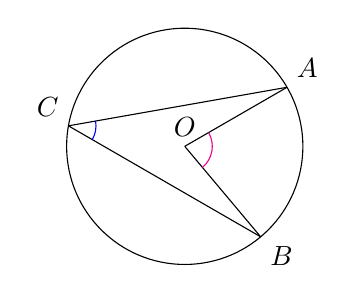
\begin{tikzpicture}[radius=1.5cm,a/.style={magenta},b/.style={blue}]
				\coordinate[label=$O$] (O) at (0,0);
				\draw (O) circle;
				\draw (O) -- ++(30:1.5cm) coordinate[label=30:$A$](A);
				\draw (O) -- ++(-50:1.5cm) coordinate[label=300:$B$](B);
				\coordinate[label=170:$C$] (C) at (170:1.5cm);
				\draw (A) -- (C) (B) -- (C);
				\tkzMarkAngle[size=0.35,a](B,O,A)
				\tkzMarkAngle[size=0.35,b](B,C,A)
			\end{tikzpicture}
			\hfill
			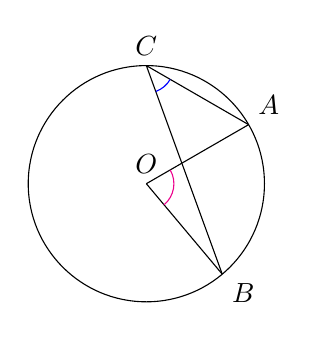
\begin{tikzpicture}[radius=1.5cm,a/.style={magenta},b/.style={blue}]
				\coordinate[label=$O$] (O) at (0,0);
				\draw (O) circle;
				\draw (O) -- ++(30:1.5cm) coordinate[label=30:$A$](A);
				\draw (O) -- ++(-50:1.5cm) coordinate[label=300:$B$](B);
				\coordinate[label=90:$C$] (C) at (90:1.5cm);
				\draw (A) -- (C) (B) -- (C);
				\tkzMarkAngle[size=0.35,a](B,O,A)
				\tkzMarkAngle[size=0.35,b](B,C,A)
			\end{tikzpicture}
			\hfill
			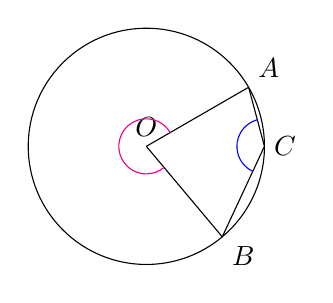
\begin{tikzpicture}[radius=1.5cm,a/.style={magenta},b/.style={blue}]
				\coordinate[label=$O$] (O) at (0,0);
				\draw (O) circle;
				\draw (O) -- ++(30:1.5cm) coordinate[label=30:$A$](A);
				\draw (O) -- ++(-50:1.5cm) coordinate[label=300:$B$](B);
				\coordinate[label=0:$C$] (C) at (0:1.5cm);
				\draw (A) -- (C) (B) -- (C);
				\tkzMarkAngle[size=0.35,a](A,O,B)
				\tkzMarkAngle[size=0.35,b](A,C,B)
			\end{tikzpicture}
			\caption{Inscribed Angle Theorem}
		\end{figure}
	\end{mdframed}
	\begin{proof}
		$ $\\	
		For the first case, we have $OA = OC = OB$. Let $\angle OCB = \angle OBC = a$ and $\angle OCB = \angle OBC = b$, then $\angle ACB = a + b$ and $\angle AOB = 2a + 2b$. \\
		For the second case, we have $OA = OC = OB$. Let $\angle OCB = \angle OBC = a$ and $\angle OCB = \angle OBC = b$, then $\angle ACB = b - a$ and  $\angle AOB = 2b - 2a$. \\
		For the third case, we have $OA = OC = OB$. Let $\angle OCB=\angle OBC = a$ and $\angle OCB = \angle OBC = b$, then  $\angle ACB = a + b$ and  $\text{reflex } \angle AOB = 2a + 2b$.

		\begin{figure}[H]
			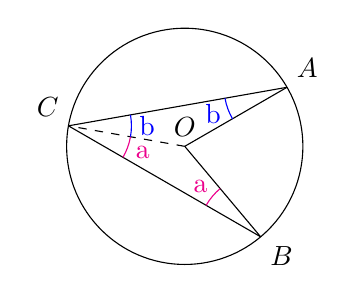
\begin{tikzpicture}[radius=1.5cm,a/.style={magenta},b/.style={blue}]
				\coordinate[label=$O$] (O) at (0,0);
				\draw (O) circle;
				\draw (O) -- ++(30:1.5cm) coordinate[label=30:$A$](A);
				\draw (O) -- ++(-50:1.5cm) coordinate[label=300:$B$](B);
				\coordinate[label=170:$C$] (C) at (170:1.5cm);
				\draw (A) -- (C) (B) -- (C);
				\draw[dashed] (O) -- (C);
				\tkzMarkAngle[size=0.8,a](B,C,O)
				\tkzLabelAngle[a](B,C,O){a}
				\tkzMarkAngle[size=0.8,a](O,B,C)
				\tkzLabelAngle[a](O,B,C){a}
				\tkzMarkAngle[size=0.8,b](C,A,O)
				\tkzLabelAngle[b](C,A,O){b}
				\tkzMarkAngle[size=0.8,b](O,C,A)
				\tkzLabelAngle[b](O,C,A){b}
			\end{tikzpicture}
			\hfill
			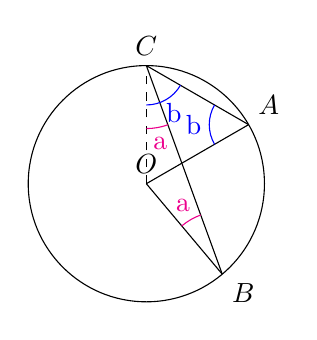
\begin{tikzpicture}[radius=1.5cm,a/.style={magenta},b/.style={blue}]
				\coordinate[label=$O$,left] (O) at (0,0);
				\draw (O) circle;
				\draw (O) -- ++(30:1.5cm) coordinate[label=30:$A$](A);
				\draw (O) -- ++(-50:1.5cm) coordinate[label=300:$B$](B);
				\coordinate[label=90:$C$] (C) at (90:1.5cm);
				\draw (A) -- (C) (B) -- (C);
				\draw[dashed] (O) -- (C);
				\tkzMarkAngle[size=0.8,a](O,C,B)
				\tkzLabelAngle[a](O,C,B){a}
				\tkzMarkAngle[size=0.8,a](C,B,O)
				\tkzLabelAngle[a](C,B,O){a}
				\tkzMarkAngle[size=0.5,b](C,A,O)
				\tkzLabelAngle[pos=0.7,b](C,A,O){b}
				\tkzMarkAngle[size=0.5,b](O,C,A)
				\tkzLabelAngle[pos=0.7,b](O,C,A){b}
			\end{tikzpicture}
			\hfill
			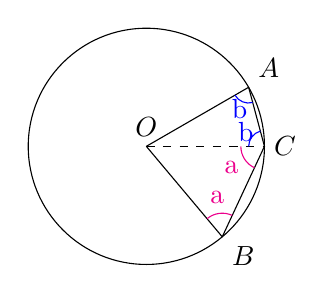
\begin{tikzpicture}[radius=1.5cm,a/.style={magenta},b/.style={blue}]
					\coordinate[label=$O$,left] (O) at (0,0);
					\draw (O) circle;
					\draw (O) -- ++(30:1.5cm) coordinate[label=30:$A$](A);
					\draw (O) -- ++(-50:1.5cm) coordinate[label=300:$B$](B);
					\coordinate[label=0:$C$] (C) at (0:1.5cm);
					\draw (A) -- (C) (B) -- (C);
					\draw[dashed] (O) -- (C);
					\tkzMarkAngle[size=0.3,a](O,C,B)
					\tkzLabelAngle[pos=0.5,a](O,C,B){a}
					\tkzMarkAngle[size=0.3,a](C,B,O)
					\tkzLabelAngle[pos=0.5,a](C,B,O){a}
					\tkzMarkAngle[size=0.2,b](O,A,C)
					\tkzLabelAngle[pos=0.3,b](O,A,C){b}
					\tkzMarkAngle[size=0.2,b](A,C,O)
					\tkzLabelAngle[pos=0.3,b](A,C,O){b}
			\end{tikzpicture}
			\caption{Proof of Inscribed Angle Theorem}
		\end{figure}
	\end{proof}

	\begin{mdframed}
		\begin{corollary}[angle in semi-circle]
				Let $AB$ be a diameter of circle, $C$ be any point on a circle. Then $\angle ACB = 90^o$ (because the angle at centre is $180^o$).
				\begin{figure}[H]
					\centering
					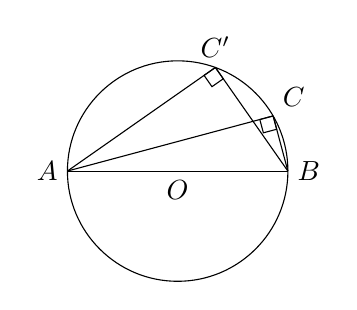
\begin{tikzpicture}[scale=0.7,radius=2cm]
						\coordinate (O) at (0,0);
						\draw (O) node[below]{$O$};
						\draw (O) circle;
						\coordinate (A) at (-2,0);
						\coordinate (B) at (2,0);
						\draw (A) node[left]{$A$} -- (B) node[right]{$B$};
						\coordinate (C) at (30:2cm);
						\coordinate (C') at (70:2cm);
						\draw (C) node[above right]{$C$};
						\draw (C') node[above] {$C'$};
						\draw (A) -- (C');
						\draw (B) -- (C');
						\draw (A) -- (C);
						\draw (B) -- (C);
						\tkzMarkRightAngle(A,C,B)
						\tkzMarkRightAngle(A,C',B)
					\end{tikzpicture}
					\caption{Angle in semi-circle}
				\end{figure}
		\end{corollary}	
	\end{mdframed}
	\begin{mdframed}
		\begin{corollary}[angle at circumference $\propto$ arc length]
			The arc is proportional to the angle at circumference (center).
		\end{corollary}
		\begin{figure}[H]
			\centering
			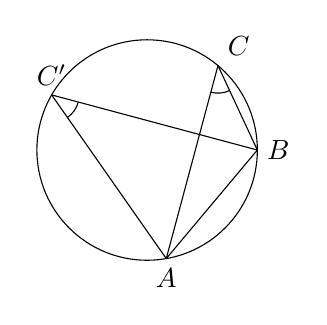
\begin{tikzpicture}[scale=0.7,radius=2cm]
				\coordinate (O) at (0,0);
				\draw (O) circle;
				\coordinate (A) at (-80:2cm);
				\coordinate (B) at (2,0);
				\draw (A) node[below]{$A$} -- (B) node[right]{$B$};
				\coordinate (C) at (50:2cm);
				\coordinate (C') at (150:2cm);
				\draw (C) node[above right]{$C$};
				\draw (C') node[above] {$C'$};
				\draw (A) -- (C');
				\draw (B) -- (C');
				\draw (A) -- (C);
				\draw (B) -- (C);
				\tkzMarkAngle[size=0.5](A,C,B)
				\tkzMarkAngle[size=0.5](A,C',B)
			\end{tikzpicture}
			\caption{Angle at circumference $\propto$ arc length}
			\label{angle propto arc}
		\end{figure}
	\end{mdframed}
\subsection{The Extended Law of Sine}
By convention, in $\Delta ABC$, the opposite side to angle $A$ is named $a$ (similarly for $B$ and $C$), $\mathcal{R}$ denotes the circumradius of $\Delta ABC$, and $r$ denotes the inradius of $\Delta ABC$.
\begin{mdframed}
	\begin{theorem}[the Extended Law of Sine]
		Given a triangle $ABC$, we have 
		\begin{equation*}
			\frac{a}{\sin A} = \frac{b}{\sin B} = \frac{c}{\sin C} = 2\mathcal{R}
		\end{equation*}
	\end{theorem}
	\begin{center}
		\begin{figure}[H]
			\centering
			\begin{tikzpicture}
				\tkzDefPoints{0/0/A,3/0/B,2/2/C}
				\tkzDefCircle[circum](A,B,C) \tkzGetPoint{O} \tkzGetLength{rayon}
				\tkzDrawCircle[dashed,R](O, \rayon pt)
				\tkzDrawPolygon(A,B,C)
				\tkzAutoLabelPoints[center=O](A,B,C)
			\end{tikzpicture}
			\caption{the Extended Law of Sine}
		\end{figure}
	\end{center}
\end{mdframed}
\begin{proof}
	Without loss of generality, we only prove $\frac{a}{\sin A} = 2\mathcal{R}$. Move $A$ to $A'$ such that $A'B$ is the diameter of the circle. Note that $\triangle ACB$ is a right-angled triangle and $\angle BA'C = \angle BAC$. We have $\frac{a}{\sin BAC} = \frac{CB}{\sin \angle BA'C} = A'B = 2\mathcal{R}$
\end{proof}
\begin{figure}[H]
	\centering
	\begin{tikzpicture}
		\tkzDefPoints{0/0/A,3/0/B,2/2/C}
		\tkzDefCircle[circum](A,B,C) \tkzGetPoint{O} \tkzGetLength{rayon}
		\tkzDrawCircle[dashed,R](O, \rayon pt)
		\tkzDrawPolygon(A,B,C)
		\tkzAutoLabelPoints[center=O](A,B,C)
		\tkzInterLC(B,O)(O,A) \tkzGetPoints{B}{A'}
		\tkzAutoLabelPoints[center=O](A')
		\tkzDrawSegment[](B,A')
		\tkzDrawSegment[](A',C)
		\tkzDrawPoint(O)
		\tkzLabelPoint[above](O){O}
		\tkzMarkRightAngle[](B,C,A')
	\end{tikzpicture}
	\caption{Proof of the Extended Law of Sine}
\end{figure}
\subsection{Relationship between Circumradius and Area}
Let $[ABC]$ denotes the area of triangle.
\begin{mdframed}
	\begin{theorem}[Area of a triangle]
		$$[ABC] = \dfrac{1}{2}ab\sin C$$.
	\end{theorem}
	\begin{figure}[H]
		\centering
		\begin{tikzpicture}
			\tkzDefPoints{0/0/A,3/0/C,2/2/B}
			\tkzDrawPolygon(A,B,C)
			\tkzDefPointsBy[projection=onto A--C](B){H}
			\tkzDrawSegment(B,H)
			\tkzLabelPoint[left](A){A}
			\tkzLabelPoint[above](B){B}
			\tkzLabelPoint[right](C){C}
			\tkzLabelPoint[below](H){H}
			\tkzLabelLine[pos=0.5,right](B,C){a}
			\tkzLabelLine[pos=0.5,below](A,C){b}
		\end{tikzpicture}
		\caption{$[ABC] = \frac{1}{2}ab \sin C$}
	\end{figure}
\end{mdframed}
\begin{proof}
	It suffices to see that $BH = a\sin C$, $AC=b$. Note that the formula also works for C greater than $90^o$ too. The proof is left as an exercise.
\end{proof}
\begin{mdframed}
			\begin{theorem}[Circumradius and Area]
				$$[ABC] = \dfrac{abc}{4\mathcal{R}}$$
			\end{theorem}
\end{mdframed}
\begin{proof}
	It follows from the extended law of sine.	
\end{proof}
\subsection{Relationship between Circumradius and Side Lengths}
Let $s$ denotes the semi-perimeter of triangle, i.e. $\frac{a+b+c}{2}$.
We state the Heron's formula without proof:
\begin{mdframed}
	\begin{theorem}[Heron's formula]
		In $\triangle ABC$, we have $$[ABC] = \sqrt{s(s-a)(s-b)(s-c)}$$.
	\end{theorem}
\end{mdframed}
Together with the previous result, we can find the circumradius of a triangle if we know all $3$ side lengths:
\begin{mdframed}
	\begin{theorem}[Circumradius and Side Lengths]
		\begin{align*}
			\mathcal{R} &= \tfrac{abc}{4\sqrt{s(s-a)(s-b)(s-c)} }
		\end{align*}
	\end{theorem}
\end{mdframed}

\section{Cyclic Quadrilateral}
Is it always possible to find a circle passing through a triangle? How about through a quadrilateral?
\begin{figure}[H]
	\centering
	\begin{minipage}{0.8\textwidth}
		\begin{tikzpicture}[scale=0.25]
			\tkzDefPoints{0/0/A,12/2/B,9/-5/C}
			\tkzDrawSegments(A,B B,C A,C)
			\tkzDefCircle[circum](A,B,C)
			\tkzGetPoint{O}
			\tkzGetLength{rayon}
			\tkzDrawCircle[dashed,R](O,\rayon pt)
		\end{tikzpicture}
		\hfill
		\begin{tikzpicture}[scale=0.25]
			\tkzDefPoints{0/0/A,12/4/B,9/8/C,-1/10/D}
			\tkzDrawSegments(A,B B,C C,D D,A)
			\tkzDefCircle[circum](A,B,C)
			\tkzGetPoint{O}
			\tkzGetLength{rayon}
			\tkzDrawCircle[dashed,R](O,\rayon pt)
		\end{tikzpicture}
	\end{minipage}
	\caption{Finding a circle passing through a triangle/quadrilateral?}	
\end{figure}
The answer to the first question is yes but the answer to the second question is no.
\subsection{Properties of Cyclic Quadrilateral}

\begin{mdframed}
	\begin{theorem}[Supplementary opposite angles]
		Opposite angles inside a cyclic quadrilateral adds up to $180^o$.
	\end{theorem}
\end{mdframed}

\begin{figure}[H]
	\centering
	\begin{tikzpicture}[scale=0.35]
		\tkzDefPoints{0/0/O,5/0/A,4/3/B,-4/3/C,-3.535/-3.535/D}
		\tkzDrawPolygon(A,B,C,D)
		\tkzDrawSegments(O,A O,C)
		\tkzDefCircle[circum](A,B,C)
		\tkzGetPoint{O}
		\tkzGetLength{rayon}
		\tkzDrawCircle[R](O,\rayon pt)

		% Label the points
		\tkzAutoLabelPoints[center=O](A,B,C,D)
		\tkzLabelPoints(O)

		% Mark the angle
		\tkzMarkAngle[color=red](A,O,C)
		\tkzLabelAngle[pos=1.5,color=red](A,O,C){$2\alpha$}
		\tkzMarkAngle[color=red](A,D,C)
		\tkzLabelAngle[pos=1.5,color=red](A,D,C){$\alpha$}
		\tkzMarkAngle[color=blue](C,O,A)
		\tkzLabelAngle[pos=1.5,color=blue](C,O,A){$2\beta$}
		\tkzMarkAngle[color=blue](C,B,A)
		\tkzLabelAngle[pos=1.5,color=blue](C,B,A){$\beta$}
	\end{tikzpicture}
	\caption{Opposite angles add up to $180^o$}
\end{figure}
\begin{proof}
	Let $\angle COA = 2\alpha$, $\text{reflex } \angle COA = 2\beta$, then $2\alpha + 2\beta = 360^o$. This implies $\alpha + \beta = 180^o$. By Inscribed Angle Theorem, we have $\angle CDA + \angle CBA = \alpha + \beta = 180$
\end{proof}
\begin{mdframed}
	\begin{corollary}
		Exterior angle equals to the opposite interior angle inside a cyclic quadrilateral.
	\end{corollary}
\end{mdframed}

\begin{mdframed}
	\begin{theorem}[Angles subtended by the same arc]
		Angles subtended by the same arc are equal.
		\begin{figure}[H]
			\centering
			\begin{tikzpicture}[scale=0.35]
				\tkzDefPoints{0/0/O,5/0/A,4/3/B,-4/3/C,-3.535/-3.535/D}
				\tkzDrawPolygon(A,B,C,D)
				\tkzDrawSegments(B,D A,C)
				\tkzDefCircle[circum](A,B,C)
				\tkzGetPoint{O}
				\tkzGetLength{rayon}
				\tkzDrawCircle[R](O,\rayon pt)

				% Label the points
				\tkzAutoLabelPoints[center=O](A,B,C,D)

				% Mark the angle
				\tkzMarkAngle[size=2.3,color=red](A,C,B)
				\tkzLabelAngle[pos=2.8,color=red](A,C,B){$\alpha$}
				\tkzMarkAngle[size=2.3,color=red](A,D,B)
				\tkzLabelAngle[pos=2.8,color=red](A,D,B){$\alpha$}
			\end{tikzpicture}
			\caption{Angle subtended by the same arc are equal}
		\end{figure}	
	\end{theorem}
\end{mdframed}
\begin{proof}
	Follows directly form Theorem \ref{angle propto arc}.
\end{proof}
\subsection{Test for Cyclic Quadrilateral}
It turns out that the mentioned $3$ properties are also tests for cyclic quadrilateral.

\begin{mdframed}
	\begin{theorem}[Test for Cyclic Quadrilateral] $ $
		\begin{itemize}
			\item Opposite angles adds up to $180^o$.
			\item Exterior angle equals the opposite interior angle.
			\item Angles subtended by the same \textbf{side} are equal.
		\end{itemize}
		This means that if \textbf{any} of the above $3$ statement is true, then the quadrilateral is a cyclic quadrilateral.
	\end{theorem}
\end{mdframed}

The proof is omitted here. Now you should have enough to solve the original problem. :)

\section{Power Chord Theorem and its Converse}

The key observation in this section is: if you have a point $P$ inside a cyclic quadrilateral $ABCD$. We have $\triangle PCD \sim \triangle PBA$. This motivates the power chord theorem.

\begin{figure}[H]
	\centering
	\begin{tikzpicture}[scale=0.35]
		\tkzDefPoints{0/0/O,5/0/A,4/3/B,-4/3/C,-3.535/-3.535/D}
		\tkzDrawPolygon(A,B,C,D)
		\tkzDrawSegments(B,D A,C)
		\tkzDefCircle[circum](A,B,C)
		\tkzGetPoint{O}
		\tkzGetLength{rayon}
		\tkzDrawCircle[R](O,\rayon pt)
		\tkzInterLL(A,C)(B,D)
		\tkzGetPoint{P}

		% Label the points
		\tkzAutoLabelPoints[center=O](A,B,C,D)
		\tkzLabelPoint[below](P){$P$}
		\tkzMarkAngle[size=1,color=red](D,C,A)
		\tkzLabelAngle[pos=1.5,color=red](D,C,A){$\alpha$}
		\tkzMarkAngle[size=1,color=red](D,B,A)
		\tkzLabelAngle[pos=1.5,color=red](D,B,A){$\alpha$}
		\tkzMarkAngle[size=1,color=blue](B,D,C)
		\tkzLabelAngle[pos=1.5,color=blue](B,D,C){$\beta$}
		\tkzMarkAngle[size=1,color=blue](B,A,C)
		\tkzLabelAngle[pos=1.5,color=blue](B,A,C){$\beta$}
	\end{tikzpicture}
	\caption{$\triangle PCD \sim \triangle PBA$}
\end{figure}

\begin{mdframed}
\begin{theorem}
	If you have a point $P$ \textbf{inside} a circle and a chord $XY$ passing through $P$, then $PX \cdot PY$ is the same regardless of what chord $XY$ is picked. The value $PX \cdot PY$ is called the power of $P$ with respect to the circle $\omega$, denoted $\Pow_\omega(P)$.
	\begin{figure}[H]
		\centering
		\begin{tikzpicture}[scale=0.35]
			\tkzDefPoints{0/0/O,5/0/A,4/3/B,-4/3/C,-2/-4.582/D,0/5/E}
			\tkzDrawSegments(B,D A,C)
			\tkzDefCircle[circum](A,B,C)
			\tkzGetPoint{O}
			\tkzGetLength{rayon}
			\tkzDrawCircle[R](O,\rayon pt)
			\tkzInterLL(A,C)(B,D)
			\tkzGetPoint{P}
			\tkzInterLC(E,P)(O,A)
			\tkzGetPoints{F}{_}
			\tkzDrawSegment(E,F)
			% Label the points
			\tkzAutoLabelPoints[center=O](A,B,C,D,E,F)
			\tkzLabelPoint[below](P){$P$}
			\tkzLabelPoint[below](O){$O$}
			\tkzDrawPoints(O)
			\tkzInterLC(P,O)(O,A)
			\tkzGetPoints{H}{G}
			\tkzAutoLabelPoints[center=O](G,H)
			\tkzDrawSegments[color=red](G,H)
		\end{tikzpicture}
		\caption{$PC \cdot PA = PE \cdot PF = PB \cdot PD$}
	\end{figure}
\end{theorem}
\end{mdframed}
\begin{proof}
	This follows from the similar triangles we just discovered. For example, note that $\triangle PEC \sim PAF$ and  $\triangle PCG \sim \triangle PAF$. The former set gives  $PE \cdot PF = PA \cdot PC$ and the later set gives $PA \cdot PC = PG \cdot PH$.
\end{proof}
\begin{mdframed}
	\begin{theorem}
		For any point $P$ \textbf{inside} $\omega$.
		\begin{equation*}
			\Pow_\omega(P) = \mathcal{R}^2 - OP^2	
		\end{equation*}
	\end{theorem}
\end{mdframed}

A different configuration motivates the power of a point $P$ outside a circle. By convention, the power of such a point is taken to be negative. This will prove convenient when discussing the radical lemma.

\begin{figure}[H]
	\centering
	\begin{tikzpicture}[scale=0.35]
		\tkzDefPoints{0/0/O,5/0/T,4/3/B,-4/3/C,0/-5/E,7/7/P}
		\tkzDefCircle[circum](T,B,C)
		\tkzGetPoint{O}
		\tkzGetLength{rayon}
		\tkzDrawCircle[R](O,\rayon pt)
		\tkzDefLine[tangent from = P](O,B) \tkzGetPoints{_}{A}
		\tkzDrawSegments(P,C)
		\tkzDrawSegments(P,E)
		\tkzInterLC(C,P)(O,A)
		\tkzGetPoints{B}{C}
		\tkzInterLC(E,P)(O,A)
		\tkzGetPoints{E}{D}
		\tkzAutoLabelPoints[center=O](P,B,C,D,E)
		\tkzDrawSegment[dashed](B,D)
		\tkzDrawSegment[dashed](C,E)
		\tkzMarkAngle[size=1,color=red](D,B,P)
		\tkzLabelAngle[pos=1.5,color=red](D,B,P){$\alpha$}
		\tkzMarkAngle[size=1,color=red](P,E,C)
		\tkzLabelAngle[pos=1.5,color=red](P,E,C){$\alpha$}
		\tkzMarkAngle[size=1,color=blue](P,D,B)
		\tkzLabelAngle[pos=1.5,color=blue](P,D,B){$\beta$}
		\tkzMarkAngle[size=1,color=blue](E,C,P)
		\tkzLabelAngle[pos=1.5,color=blue](E,C,P){$\beta$}
	\end{tikzpicture}
	\caption{$\triangle PBD \sim \triangle PEC$}
	\label{power chord theorem 2}
\end{figure}
\begin{mdframed}
	\begin{theorem}
	If you have a point $P$ \textbf{outside} a circle and a chord $XY$ passing through $P$, then $PX \cdot PY$ is the same regardless of what chord $XY$ is picked. The value $-|PX \cdot PY|$ is called the power of $P$ with respect to the circle $\omega$, denoted $\Pow_\omega(P)$.
		\begin{figure}[H]
			\centering
			\begin{tikzpicture}[scale=0.35]
				\tkzDefPoints{0/0/O,5/0/T,4/3/B,-4/3/C,0/-5/E,7/7/P}
				\tkzDefCircle[circum](T,B,C)
				\tkzGetPoint{O}
				\tkzGetLength{rayon}
				\tkzDrawCircle[R](O,\rayon pt)
				\tkzDefLine[tangent from = P](O,B) \tkzGetPoints{_}{A}
				\tkzDrawSegments(P,A)
				\tkzDrawSegments(P,C)
				\tkzDrawSegments(P,E)
				\tkzInterLC(C,P)(O,A)
				\tkzGetPoints{B}{C}
				\tkzInterLC(E,P)(O,A)
				\tkzGetPoints{E}{D}
				\tkzAutoLabelPoints[center=O](P,A,B,C,D,E)
				\tkzInterLC(O,P)(O,A) \tkzGetPoints{G}{H}
				\tkzDrawSegment[color=red](P,G)
				\tkzDrawPoint(O)
				\tkzAutoLabelPoints[center=O](H,G)
				\tkzLabelPoint[below](O){$O$}
			\end{tikzpicture}
			\caption{$PB \cdot PC = PD \cdot PE = PA^2$}
		\end{figure}
	\end{theorem}
\end{mdframed}

\begin{proof}
	Similar to the one above.
\end{proof}

\begin{mdframed}
	\begin{theorem}
		For any point $P$ \textbf{outside} $\omega$.
		\begin{equation*}
			\Pow_\omega(P) = \mathcal{R}^2 - OP^2	
		\end{equation*}
	\end{theorem}
\end{mdframed}

\begin{mdframed}
	\begin{theorem}
		$\Pow_\omega(P)$ \textbf{on} the circle $\omega$ is defined to be $0$. (Why does this makes sense?)
	\end{theorem}
\end{mdframed}

\begin{mdframed}
	\begin{theorem}
		For any point $P$ on $\omega$.
		\begin{equation*}
			\Pow_\omega(P) = \mathcal{R}^2 - OP^2	
		\end{equation*}
	\end{theorem}
\end{mdframed}

Hence $\Pow_\omega(P) = \mathcal{R}^2 - OP^2$ always hold no matter whether $P$ lies inside, on, or outside the circle, thanks to the power outside circle being negative.

\subsection{Converse of Power Chord Theorem}

In fact, the converse of power chord theorem is also true.	
\begin{mdframed}
	\begin{theorem}[Converse of the Power Chord Theorem]
		Let $A,B,X,Y$ be four distinct points in the plane and let lines  $AB$ and  $XY$ intersect at $P$. Suppose that either $P$ lies in both of the segments $\overline{AB}$ and $\overline{XY}$, or in neither segment. If $PA \cdot PB = PX \cdot PY$, then $A, B, X, Y$ are concyclic.
	\end{theorem}
\end{mdframed}
This serves as another test for cyclic quadrilateral. The proof is omitted here.

\subsection{Another proof of the Pythagoras Theorem}
Consider the following figure. We know that radius of a circle $OA$ is perpendicular to the tangent through $A$.
\begin{figure}[H]
	\centering
	\begin{tikzpicture}[scale=0.3]
		\tkzDefPoints{0/0/O,5/0/T,4/3/B,-4/3/C,0/-5/E,7/7/P}
		\tkzDefCircle[circum](T,B,C)
		\tkzGetPoint{O}
		\tkzGetLength{rayon}
		\tkzDrawCircle[R](O,\rayon pt)
		\tkzDefLine[tangent from = P](O,B) \tkzGetPoints{_}{A}
		\tkzDrawSegments(P,O O,A)
		\tkzDrawSegments(P,A)
		\tkzAutoLabelPoints[center=O](P,A)
		\tkzDrawPoint(O)
		\tkzLabelPoint[above](O){O}
	\end{tikzpicture}
	\caption{Another proof of the Pythagoras Theorem}
\end{figure}
Then two ways of calculating the power of $P$ with respect to the circle: \\ $\Pow_\omega(P) = \mathcal{R}^2 - OP^2 = AP^2$ gives rise to the Pythagoras Theorem.

\section{Properties of Tangent to Circle}
\subsection{Angle in Alternate Segment}
\begin{mdframed}
	\begin{theorem}[Angle in Alternate Segment]
		In any circle, the angle between a chord and a tangent through one of the end points of the chord is equal to the angle in the alternate segment.
		\begin{figure}[H]
			\centering
			\begin{tikzpicture}[scale=0.4]
				\tkzDefPoints{0/0/O,5/0/T,4/3/B,-4/3/C,0/-5/E,7/7/P}
				\tkzDefCircle[circum](T,B,C)
				\tkzGetPoint{O}
				\tkzGetLength{rayon}
				\tkzDrawCircle[R](O,\rayon pt)
				\tkzDefLine[tangent from = P](O,B) \tkzGetPoints{_}{A}
				\tkzInterLC(C,P)(O,A)
				\tkzGetPoints{B}{C}
				\tkzInterLC(E,P)(O,A)
				\tkzGetPoints{E}{D}
				\tkzAutoLabelPoints[center=O](C,E)
				\tkzDefTangent[at=D](O)
				\tkzGetPoint{h}
				\tkzDrawLine[add=4 and 4](D,h)
				\tkzDrawSegment(C,D)
				\coordinate (B'') at ($(D)!5cm!(h)$);
				\tkzLabelPoint[above](B''){$\textcolor{black}{B''}$}
				\coordinate (B''') at ($(h)!5cm!(D)$);
				\tkzLabelPoint[below](B'''){$\textcolor{black}{B'''}$}
				\tkzDrawSegments[](D,E C,E)
				\tkzMarkAngle[size=1](E,C,D)
				\tkzLabelAngle[pos=1.5](E,C,D){$\beta'$}
				\tkzMarkAngle[size=1](E,D,B''')
				\tkzLabelAngle[pos=1.5](E,D,B'''){$\beta'$}
				\tkzLabelPoint[right](D){$\textcolor{black}{B'}$}
			\end{tikzpicture}
			\caption{Angle in Alternate Segment}
		\end{figure}
	\end{theorem}
\end{mdframed}
	\begin{proof}
		Recall the configuration in Theorem \ref{power chord theorem 2}. Imagine if $B$ gets increasingly close to $D$ at $B'$ such that $B'D$ becomes the tangent to the circle at $D$. Label the new line $B''B'''$ as shown in the second figure. Then $\angle B''DP = \angle B'CE$ since exterior angle of cyclic quadrilateral is the same as the opposite interior angle. Finally, $\angle B''DP = \angle DEB'''$ concludes the proof.
		\begin{figure}[H]
			\centering
			\begin{tikzpicture}[scale=0.4]
				\tkzDefPoints{0/0/O,5/0/T,4/3/B,-4/3/C,0/-5/E,7/7/P}
				\tkzDefCircle[circum](T,B,C)
				\tkzGetPoint{O}
				\tkzGetLength{rayon}
				\tkzDrawCircle[R](O,\rayon pt)
				\tkzDefLine[tangent from = P](O,B) \tkzGetPoints{_}{A}
				\tkzInterLC(C,P)(O,A)
				\tkzGetPoints{B}{C}
				\tkzInterLC(E,P)(O,A)
				\tkzGetPoints{E}{D}
				\tkzAutoLabelPoints[center=O](C,E)

				\tkzAutoLabelPoints[center=O](B)
				\coordinate[label=60:$P$] (P) at ($(D)!-2cm!(E)$);
				\tkzDrawLine[add=0.3 and 0](D,E)
				\tkzDrawSegment(B,C)
				\tkzDrawSegment(B,D)
				\tkzDrawSegment(C,E)
				\tkzMarkAngle[size=1,color=blue](P,D,B)
				\tkzLabelAngle[pos=1.5,color=blue](P,D,B){$\beta$}
				\tkzMarkAngle[size=1,color=blue](E,C,B)
				\tkzLabelAngle[pos=1.5,color=blue](E,C,B){$\beta$}
			\end{tikzpicture}
			\hfill
			\begin{tikzpicture}[scale=0.4]
				\tkzDefPoints{0/0/O,5/0/T,4/3/B,-4/3/C,0/-5/E,7/7/P}
				\tkzDefCircle[circum](T,B,C)
				\tkzGetPoint{O}
				\tkzGetLength{rayon}
				\tkzDrawCircle[R](O,\rayon pt)
				\tkzDefLine[tangent from = P](O,B) \tkzGetPoints{_}{A}
				\tkzInterLC(C,P)(O,A)
				\tkzGetPoints{B}{C}
				\tkzInterLC(E,P)(O,A)
				\tkzGetPoints{E}{D}
				\tkzAutoLabelPoints[center=O](C,E)

				\tkzAutoLabelPoints[center=O](B)
				\coordinate[label=60:$P$] (P) at ($(D)!-2cm!(E)$);
				\tkzDrawLine[add=0.3 and 0](D,E)
				\tkzDrawSegment(B,C)
				\tkzDrawSegment(B,D)
				\tkzLabelPoint[right](D){$D,\textcolor{red}{B'}$}


				\tkzDefTangent[at=D](O)
				\tkzGetPoint{h}
				\tkzDrawLine[add=4 and 4,color=red](D,h)
				\tkzDrawSegment[color=red](C,D)
				\coordinate (B'') at ($(D)!5cm!(h)$);
				\tkzLabelPoint[above](B''){$\textcolor{red}{B''}$}
				\coordinate (B''') at ($(h)!5cm!(D)$);
				\tkzLabelPoint[below](B'''){$\textcolor{red}{B'''}$}

				\tkzDrawSegments[color=red](D,E C,E)
				\tkzMarkAngle[size=1,color=red](E,C,D)
				\tkzLabelAngle[pos=1.5,color=red](E,C,D){$\beta'$}

				\tkzLabelAngle[pos=1.5,color=red](P,D,B''){$\beta'$}
				\tkzMarkAngle[size=1,color=red](P,D,B'')

				\tkzMarkAngle[size=1,color=red](E,D,B''')
				\tkzLabelAngle[pos=1.5,color=red](E,D,B'''){$\beta'$}
			\end{tikzpicture}
			\caption{Proof of Angle in Alternate Segment}
		\end{figure}
	\end{proof}
	\subsection{Other Properties of Tangents}

	\begin{mdframed}
		\begin{theorem}[Equal Tangents]
			The two tangents of a point outside the circle $P$ to the circle has equal length.
			\begin{figure}[H]
				\centering
				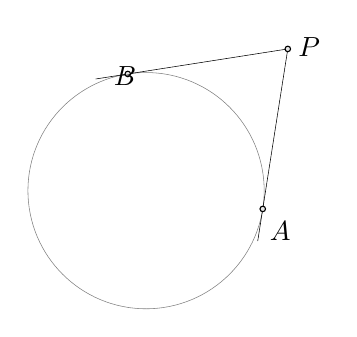
\begin{tikzpicture}[scale=0.3]
					\tkzDefPoints{0/0/O, 5/0/A, 6/6/P}
					\tkzDrawCircle(O,A)
					\tkzDefTangent[from=P](O,A) \tkzGetPoints{A}{B}
					\tkzDrawSegments[add=0 and .2](P,A P,B)
					\tkzDrawPoints(A,P,B)
					\tkzAutoLabelPoints[center=O](P,A,B)
				\end{tikzpicture}
				\caption{Equal Tangents}
			\end{figure}
		\end{theorem}
		\begin{proof}
			$\Pow_\omega(P) = PA^2 = PB^2$
		\end{proof}
	\end{mdframed}

	\begin{mdframed}
		\begin{theorem}
			Let $P$ be a point outside circle and $A$ and $B$ be the two points of tangency from $P$ to the circle, then $OABP$ is concyclic.
			\begin{figure}[H]
				\centering	
				\begin{tikzpicture}[scale=0.3]
					\tkzDefPoints{0/0/O, 5/0/A, 6/6/P}
					\tkzDrawCircle(O,A)
					\tkzDefTangent[from=P](O,A) \tkzGetPoints{A}{B}
					\tkzDrawSegments[add=0 and .2](P,A P,B)
					\tkzDrawSegments(O,A O,B)
					\tkzDrawPoints(O,A,P,B)
					\tkzAutoLabelPoints[center=O](P,A,B)
					\tkzLabelPoints(O)
					\tkzDefCircle[circum](O,A,B)
					\tkzGetPoint{O'}
					\tkzGetLength{rayon}
					\tkzDrawCircle[dashed,R,color=red](O',\rayon pt)
				\end{tikzpicture}
				\caption{OABP is concyclic}
			\end{figure}
		\end{theorem}
	\end{mdframed}
	\begin{proof}
		$\angle OBP + \angle OAP = 180^o$
	\end{proof}
	\newpage
	\section{Example Problems}
	\begin{question}
		(Prelim 2020 Q6) In $\triangle ABC, AB = 6, BC = 7, CA = 8$. Let $D$ be the mid-point of minor arc $AB$ on the circumcentre of $\triangle ABC$. Find $AD^2$.
	\end{question}
	\vfill
	\begin{question}
		(Prelim 2022 Q16) $ABCD$ is a parallelogram with $\angle B$ acute. A circle is tangent to $BC$, $CD$ and $DA$. The circle intersects $AC$ at $M$ and $N$, where $M$ is closer to $A$ than $N$. If $AM = 9$, $MN = 16$ and $NC = 2$, find the area of $ABCD$.
	\end{question}
	\vfill
	\newpage
	\section{Practice Problems}
	\begin{question}
		(Prelim 2023 Q17) $ABCD$ is a square. $P$ is a point inside $ABCD$ such that $\angle APD + \angle BPC = 180^o$ and  $\angle BPC$ is acute.  If $PB = 3$ and $PC = 4$, find $BC$.
	\end{question}
	\vfill
	\begin{question}
		(Prelim 2021 Q12) $OABC$ is a trapezium with $OC \parallel AB$ and $\angle AOB = 37^o$	. Furthermore, $A,B,C$ all lie on the circumference of a circle centered at $O$. The perpendicular bisector of $OC$ meets $AC$ at $D$.
	\end{question}
	\vfill
	\newpage
	\begin{question}
		(Prelim 2018 Q13) Let $O$ be the circumcentre of $\triangle ABC$. Suppose $AB = 1$ and $AO = AC = 2$. $D$ and $E$ are points on the extensions of $AB$ and $A C$ respectively such that $OD = OE $ and $BD = \sqrt{2} EC$. Find the value of $OD^2$.
	\end{question}
	\vfill
	\begin{question}
		(Prelim 2018 Q16) $ABCD$ is a cyclic quadrilateral with $AC=56$, $BD=65$, $BC>DA$ and $\frac{AB}{BC} = \frac{CD}{DA}$. Find the ratio of the area of $\triangle ABC$ to the area of $\triangle ADC$.
	\end{question}
	\vfill
	\newpage
	\begin{question}
		(Prelim 2016 Q20) In $\triangle ABC$, $P$ and $Q$ are points on $AB$ and $AC$ respectively such that $AP:PB=8:1$ and $AQ:QC=15:1$.  $X$ and $Y$ are points on $BC$ such that the circumcircle of $\triangle APX$ is tangent to both $BC$ and $CA$, while the circumcircle of  $\triangle AQY$ is tangent to both $AB$ and $BC$. Find $\cos BAC$.
	\end{question}
	\vfill
	\begin{question}
		(Prelim 2012 Q13) $A B C D$ is a convex quadrilateral in which $A C$ and $B D$ meet at $P$. Given $P A=1$, $P B=2, P C=6$ and $P D=3$. Let $O$ be the circumcentre of $\triangle P B C$. If $O A$ is perpendicular to $A D$, find the circumradius of $\triangle P B C$.
	\end{question}
	\vfill
\end{document}

